%\documentclass{article}
\documentclass[paper=a4, fontsize=11pt]{scrartcl}

\usepackage{graphicx}
\usepackage{longtable}
\usepackage{amsmath}
\usepackage[T5]{fontenc}                           
\usepackage[utf8]{inputenc}
\usepackage{multirow}
\usepackage{listings}
\usepackage{color}
\usepackage{hyperref}

\definecolor{codegreen}{rgb}{0,0.6,0}
\definecolor{codegray}{rgb}{0.5,0.5,0.5}
\definecolor{codepurple}{rgb}{0.58,0,0.82}
\definecolor{backcolour}{rgb}{0.95,0.95,0.92}
 
\lstdefinestyle{mystyle}{
    backgroundcolor=\color{backcolour},   
    commentstyle=\color{codegreen},
    keywordstyle=\color{magenta},
    numberstyle=\tiny\color{codegray},
    stringstyle=\color{codepurple},
    basicstyle=\footnotesize,
    breakatwhitespace=false,         
    breaklines=true,                 
    captionpos=b,                    
    keepspaces=true,                 
    numbers=left,                    
    numbersep=5pt,                  
    showspaces=false,                
    showstringspaces=false,
    showtabs=false,                  
    tabsize=2
}
\lstset{style=mystyle}

\begin{document}

\title{The Stony Brook Glad All Over Machine\\ Project Proposal}
\author{Trung Nguyen - 111752939
\\Anh Quang Do - 110922124
\\Nam Nguyen - 111171365}
\date{\today}
\maketitle
  
\section{Background}
\subsection{Music information retrieval (MIR)}

MIR is an interdisciplinary research that lies on the edges of musicology, psychology, signal processing, and machine learning. 
%Applications of MIR can be listed as follows:
%
%\begin{itemize}
%\item Music recommendation and annotation
%\item Automatic classification of genre, mood, artists, etc.
%\item Automatic music transcription
%\item Music generation
%\end{itemize}

%In our project, we focus on learning to rank/group the performance of vocal singing.

Basic of a MIR system, including segmentation, feature extraction, analysis is represented as in the figure below.
\begin{center}
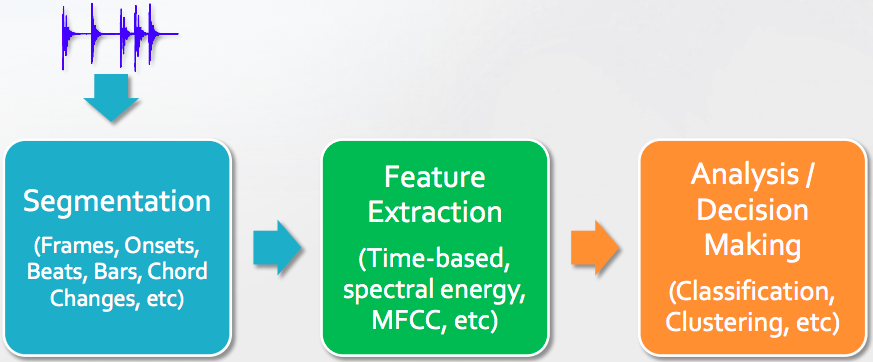
\includegraphics[scale=0.2]{img/method.png}\\
\textit{Basic of a MIR system}\\
\end{center}

\subsection{Automatic Evaluation of Karaoke Singing}
%Karaoke is a popular form of singing entertainment, rooted from Japan. 
Many of nowaday karaoke systems have a scoring feature to evaluate singers' performance. However, these rating is poorly constructed and not matched with human rating. 
%Though speech processing is a very developed field of studies and techonologies, its approach is not suitable for singing voice because singing voice differs from speech in its intensity and dynamic range and because singing voice usually comes with a non stationary background music signal.

In this project, we focus on the vocal quality of the singing and train the machine to distinguish between good and poor singing. This can be done by recalling features of the singing, such as enthusiasm, emotion, pitch, volume, rythm, melodic similarity measures, etc.

\subsection{Feature representation}
Music analysis often requires some summarising and is achieved by feature extraction. One common feature extracted is the Mel-Frequency Cepstral Coefficient (MFCC).

\subsubsection{Feature extraction}

%To evaluate a piece of singing, we would like to combine both the score-based and machine-learned ranking methods. We first identify the perception which makes a piece of singing good or bad; it can be the enthusiasm of singers, which is mostly represented by intensity of the singings, or it can be the pitch interval, the vibrato, etc., or both. Then, we then link this perception to appropriate acoustic features. Alternatively, we can do a feature importance analysis among these acoustic features.

There are many features that can be extracted from music signal. These features can be categorized into: reference features, content-based features and text-based features. Reference features can be those relating to social interactions, e.g. followers, performance rating in, for example, soundcloud. Text-based features includes lyrics, interview, etc. Our approach will be based on content-based features, extracted from the wave signal, e.g. pitch, rythm, etc. and we might use reference features as ground truth for our machine-learned ranking method.

\subsubsection{Mel-Frequency Cepstral Coefficient (MFCC) }
The content-based features are calculated from low-level signal features (sometime refered as extraction methods), the most important of which is MFCC. MFCC and its derived features (such as "anchor space"[1]) have been shown to give good performance for a variety of audio classification tasks. MFCCs capture the short-time spectral shape, which carries information about instrumental timbres or the quality of a singing. 

%MFCCs are commonly derived as follows:

%\begin{itemize}
%
%\item Take the Fourier transform of (a windowed excerpt of) a signal.
%\item Map the powers of the spectrum obtained above onto the mel scale, using triangular overlapping windows.
%\item Take the logs of the powers at each of the mel frequencies.
%\item Take the discrete cosine transform of the list of mel log powers, as if it were a signal.
%\end{itemize}

MFCCs are increasingly finding uses in music information retrieval applications such as genre classification, audio similarity measures, etc.

%\subsubsection{Music perception}
%%Human can easily distinguish between music and noise. Physically, music is ordered and patterned sound waves, produced by harmonic vibrations from the source. 
%
%The major attibutes of music are as follows:
%
%\begin{itemize}
%\item The pitch value is determined by the wavelength of the sound signal. High-pitched tones have short wavelengths, while low-pitched tones have long wavelengths.
%\item Intensity, or loudness is to the magnitude of acoustic waves. High-magnitude sound carries more energy than low-magnitude sound.
%item Duration refers to the amount of time in which a musical note sustain.
%\item Timbre refers to different harmonics, created by different source, e.g. piano vs. violin. 
%\end{itemize}


\section{Related work}
Music similarity metrics is a research aiming to calculate the similarity between songs or artists, comparing their performance. In [1], authors employ a feature, derived from MFCC, called 'anchor space', which uses musical categories and well-known anchor artists as convenient reference points for describing features of the music. It is inspired by a fold wisdom such as "Jeff Buckley sounds like Van Morrison meets Led Zeppelin, but more folky." Other approaches for song similarity are to embed songs into a Euclidian metric space and do some distance-based analysis and clustering [3].

For evaluation of karaoke singing, there is an approach based on the perception of singing enthusiasm [4]. The authors argue that karaoke is the form of entertainment for amateur so enthusiasm is a good criteria to evaluate them. They identified three acoustic features relevant to such perception: A weighted power, "fall-down", and vibrato extent, developed a system for evaluating singing enthusiasm, and obtained a correlation coefficient of 0.65 between the system output and human evaluation. In our point of view, their method can be considered as score-based ranking. In [5], the authors proposed a score combination from pitch-based, volume-based, and rhythm-based rating, with a reference specified karaoke song to evaluate a piece of singing. This approach is also score-based ranking. In [6], the authors used HMM as a statistical music recognition model for automatic scoring of karaoke computer games. The musical features they employed are Pitch \& Pitch Error, Accent, Zero-Crossing Rate, Root-Mean-Squared Energy.

Another effort for analyzing the singing voice is made in [7], in which the authors reported good results of a system for classifying "good" and "poor" singing based on SVM. In [8], the authors proposed a categorization and segmentation system for singing voice expression using pre-defined rules and HMM. There is another approach for automatic scoring of singing voice based on melodic similarity measures [9]. In [10], a method of evaluating singing skills that does not require score information is represented. The authors used pitch interval accuracy and vibrato as acoustic features to evaluate singing. The approach was then tested by a 2-class (good/poor) classification test with 600 song sequences, and achieved an average classification rate of 83.5\%. There is an approach for song classification based on perception of emtion [11].

\section{Our Approach}

\subsection{Dataset}
This project requires a large amount of audio data. For this reason, we visited several karaoke websites to look for recording data and among them, \textit{Redkaraoke} was found to be one of the largest sites for online recording worldwide which was created in 2007 and has more than 70000 songs (normally a karaoke website has ~15000 songs). Its users are also very diverse in regions. Therefore we think this website can provide good data for our purpose. 

We first chose a song, which is \textit{"My heart will go on"} by Celine Dion for our experiment. The reasons behind this choice is that it is one of the most popular and most recorded songs, its level of difficulty is relatively high, and we all like this song so we don't mind hearing it over and over again. The url for this song is:  \url{https://www.redkaraoke.com/karaoke/celine-dion/my-heart-will-go-on/11827}

We then built a scraper using \textit{BeautifulSoup4} library to extract the recordings and users' information. For this \textit{"My heart will go on"} song, we were able to sucessfully extracted around  4000 recordings, around half are .mp3 files and the rest are .mp4 files. We first downloaded all the .mp3 files, which take around 7.5GB of data storage. The scraper we built can extract information for other songs as well, but we think this amount of data is enough for us to experiment and we can always extract information for more songs whenever needed.

Aside from the audio files, text information from the recordings and the users were also extracted and saved as a csv file shown below:
 
 \begin{center}
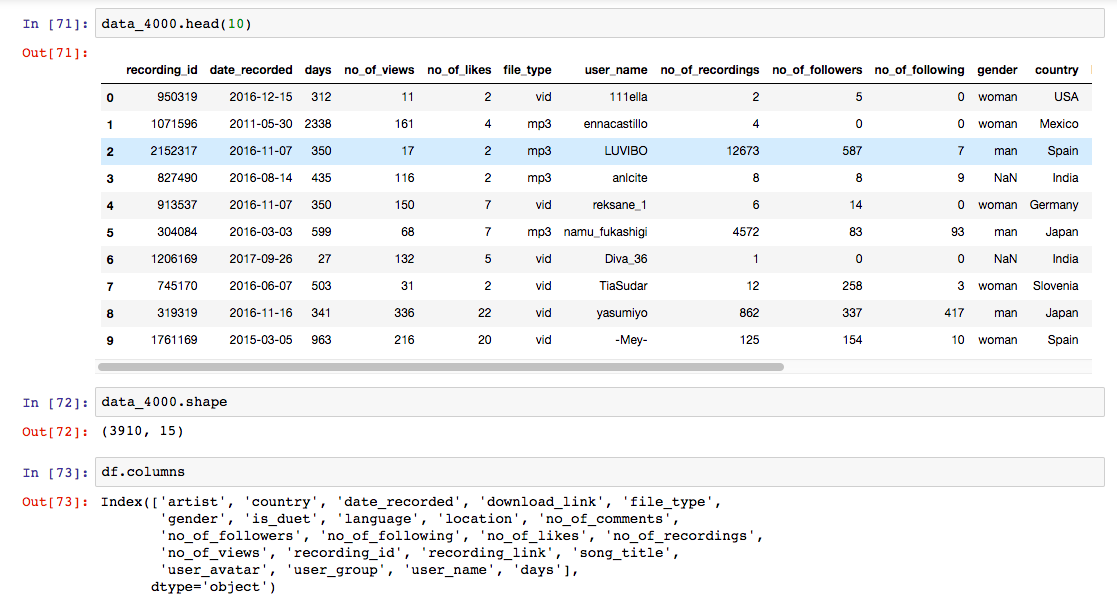
\includegraphics[scale=0.235]{img/1.png}\\
\textit{Extracted songs and users' information}\\
\end{center}

\subsection{Tools and libraries}

There are many tools available for audio analysis in python, many of which are available to be evaluated in [2]. Among them, we chose the \textit{librosa} library to experiment because of its instruction availability. 


\subsection{Method and Experiment}

Our workflow follows the \textit{Music information retrieval process} presented in section 1.1: First we segment the music (since each audio file has different length) then extract the feature and finally use machine learning methods to evaluate/group the recordings.

We had experimented extracting the 20 MFCC features from a sample audio file in our dataset. We will continue to find more information about these features to decide which are useful for our problems.

\begin{center}
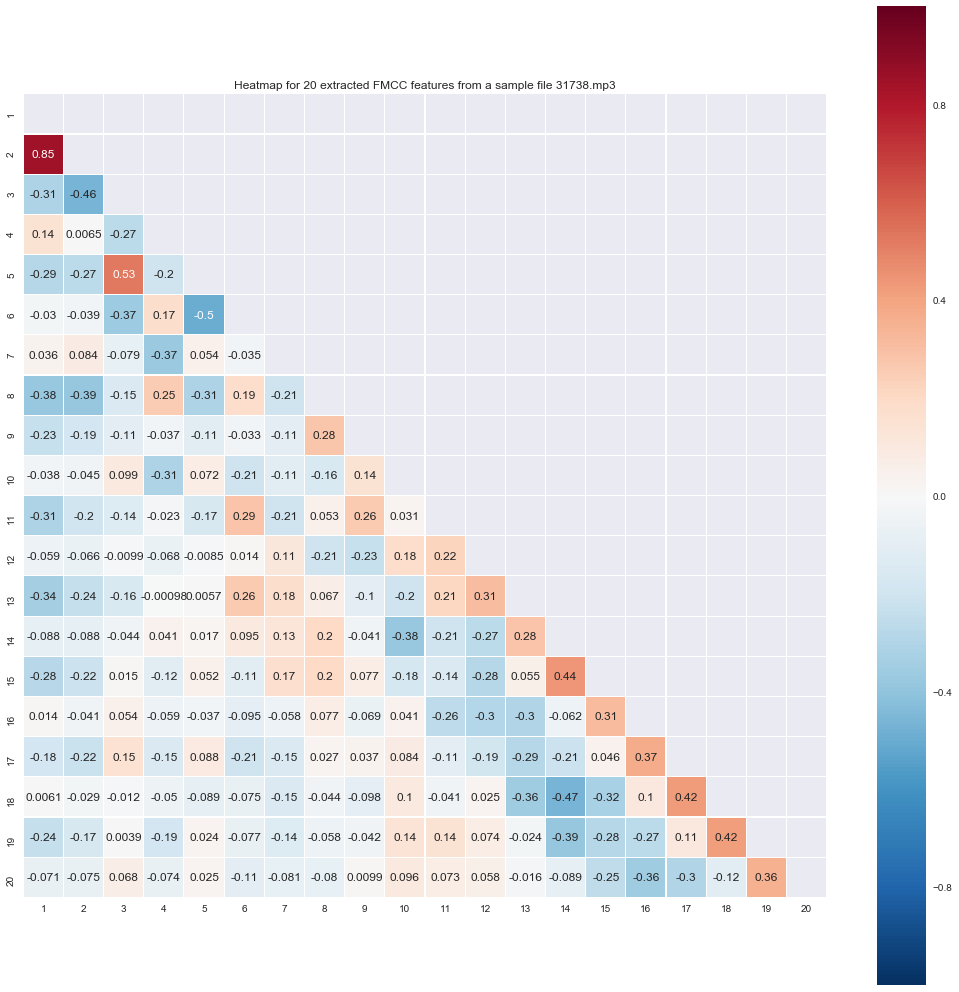
\includegraphics[scale=0.27]{img/2.png}\\
\textit{Heat map of 20 MFCC features extracted from a sample audio file in our dataset}\\
\end{center}

Once this step is finished, we may experiment building our model based Metric Learning to Rank [12] to automatically learn the distance metric, and compare it with distance in Euclidian metric space. This distance metric that have been learned will then be used in a learning to rank algorithm, based on Structural SVM.

Besides we want to extract the information not only from the audio files (content-features), but also from the information in the we retrieved (reference feature). These features may act as the groundtruth for our model. One metric which we find interesting is the number of likes.  Below is the statistics for the average number of likes in each time frame of 100 days. Except from some outliers (which turns out to be good singers who records several recordings in a short time), the average numbers of like is quite stable. From this analysis, we may conclude that this information may not heavily dependent on the recording's age, and therefore the number of likes may be good good for evaluating whether a recording is good or bad.

\begin{center}
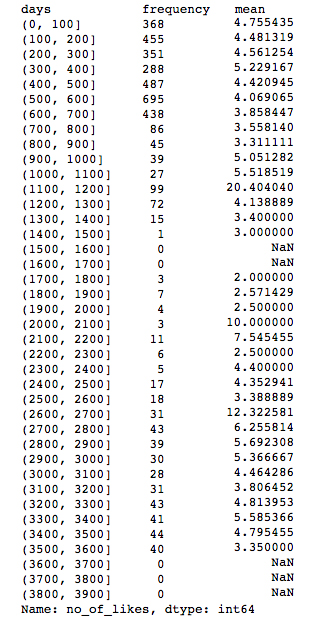
\includegraphics[scale=0.3]{img/3.jpg}\\
\textit{Average number of likes for the recordings in each time frame of 100 days}\\
\end{center}

Separating the vocal and non-vocal segments of song as a preprocessing step is also considered. However this turns out to be a hard problem: as oppose to professional multi-channel audio recordings, our mp3 files only have 1-2 channels which is very difficult to separate the vocal and non-vocal segments. We will continue to find if there is a solution for this problem.

%Our workflow would be as follows. First, we will separate the vocal and non-vocal segments of song. Then, we extract the acoustic features from the singing part. Next, 
%
%we will build our model based Metric Learning to Rank [12] to automatically learn the distance metric, rather than embed our songs in a Euclidian metric space. This distance metric that have been learned will then be used in a learning to rank algorithm, based on Structural SVM.
%
% In [12], the authors derived a general metric learning algorithm which optimizes the permutation of data, which is the output of a learning to rank algorithm, induced by distances in the learned metric. In other words, they proposed a metric learning algorithm optimized for rank-based loss function.

%In this project, we do the feature extraction based on available toolboxes instead of doing low-level signal processing and transform (FFT, Wavelet, etc.). Some of toolboxes which could be used are described as follows:

%\begin{itemize}
%\item Aubio: A library that extracts high level features such as beat tracking, tempo, melody.
%\item Timbre Toolbox: A Matlab toolbox for high and low level feature extraction, providing different set of features to the MIR Toolbox, specifically made efficient for identifying timbre.
%\item YAAFE: A library for Low level feature extraction, designed for computational efficiency and batch processing, written in C++ with a CLI and bindings for Python and Matlab.
%\item pyAudioAnalysis: An open Python library that provides a wide range of audio-related functionalities focusing on feature extraction, classification, segmentation and visualization issues.
%\item The Echo Nest Analyze API: An online system which can receive a song sent by users, analyze the acoustics and provide features to characterize global properties of the songs.
%\end{itemize}

\subsection{Evaluation}

\begin{thebibliography}{99}
\bibitem[1]{p3} E.L. Hall, J.B.K. Tio, C.A. McPherson, F.A. Sadjadi
\newblock Measuring Curved Surfaces for Robot Vision
\newblock \emph{Computer} Vol.15, no. 12, pp. 42-54 (1982)

\bibitem[2]{p3} Z.Zhang
\newblock Flexible new technique for camera calibration
\newblock IEEE Transactions on Pattern Analysis and Machine Intelligenc, vol. 22, no. 11, pp. 1330-1334 (2000)

\bibitem[3]{p3} J.Bouguet
\newblock Camera calibration toolboxfor MATLAB (2010)
\newblock http://www.vision.caltech.edu/bouguetj/calib doc/

\bibitem[4]{p3} J.Falcao, N.Hurtos
\newblock Projector-camera calibration toolbox (2009)
\newblock http://code.google.com/p/procamcalib/

\bibitem[5]{p2} Paul M.Griffin, Lakshmi S.Narasimhan and Sound R. Yee
\newblock Generation of uniquely encoded light patterns for range data acquisition
\newblock \emph{Pattern Recognition} Vol. 25, pp. 609-616 (1992)

\bibitem[6]{p1} Yi-Chih Hsieh
\newblock Decoding structured light patterns for three-dimensional imaging systems
\newblock \emph{Pattern Recognition} Vol. 34, pp. 343-349 (2001) 

\end{thebibliography}

\end{document}